\subsection{Data-Driven Estimation of Lost Lepton from W+jets and Top}
\label{sect:intro}
After applying the selection cuts, described in detail in Section~\ref{sect:cuts}, the background 
events are dominated by $t\bar t$ events. Among all decay channels of top pair system, 
it is mainly the semi-leptonic decay which contributes to the background. 
This can be understood because genuine neutrino is produced in the semi-leptonic decay of 
top pair system, $t\bar t\rightarrow W^+bW^-\bar b\rightarrow b\bar bl\nu_ljj$, 
which can pass the $M_{T2}$ cut while the full-hadronic decay products, $t\bar t\rightarrow W^+bW^-\bar b\rightarrow b\bar bjjjj$, do not contain any neutrino.
This section describes a method to estimate the backgrounds from the leptonic decay of $W$ bosons, 
either from prompt production in $W+$jets events or from $W$ bosons produced in single top and 
top pair events, shown as $t(\bar t)$ for simplicity. The lepton is considered to be electron or muon.\\
Although the leptons are vetoed in the main analysis, but there are still some background 
from $W\rightarrow l\nu_l$, referred to as lost lepton background events, 
contributing to the full-hadronic analysis. This is due to the acceptance cuts or 
inefficiencies in the lepton isolation and identification criteria.\\
In order to estimate the backgrounds due to the lost lepton events, all selection cuts are applied except
 lepton veto which is inverted. The distribution of the $p_T$ of the leptons in the events 
with exactly one lepton, being either electron or muon, are shown in 
Figure~\ref{fig:pt}, where it can be seen that the number of MC events are greater than the 
observed number of data events.\\
\begin{figure}[htbp] 
\centering
%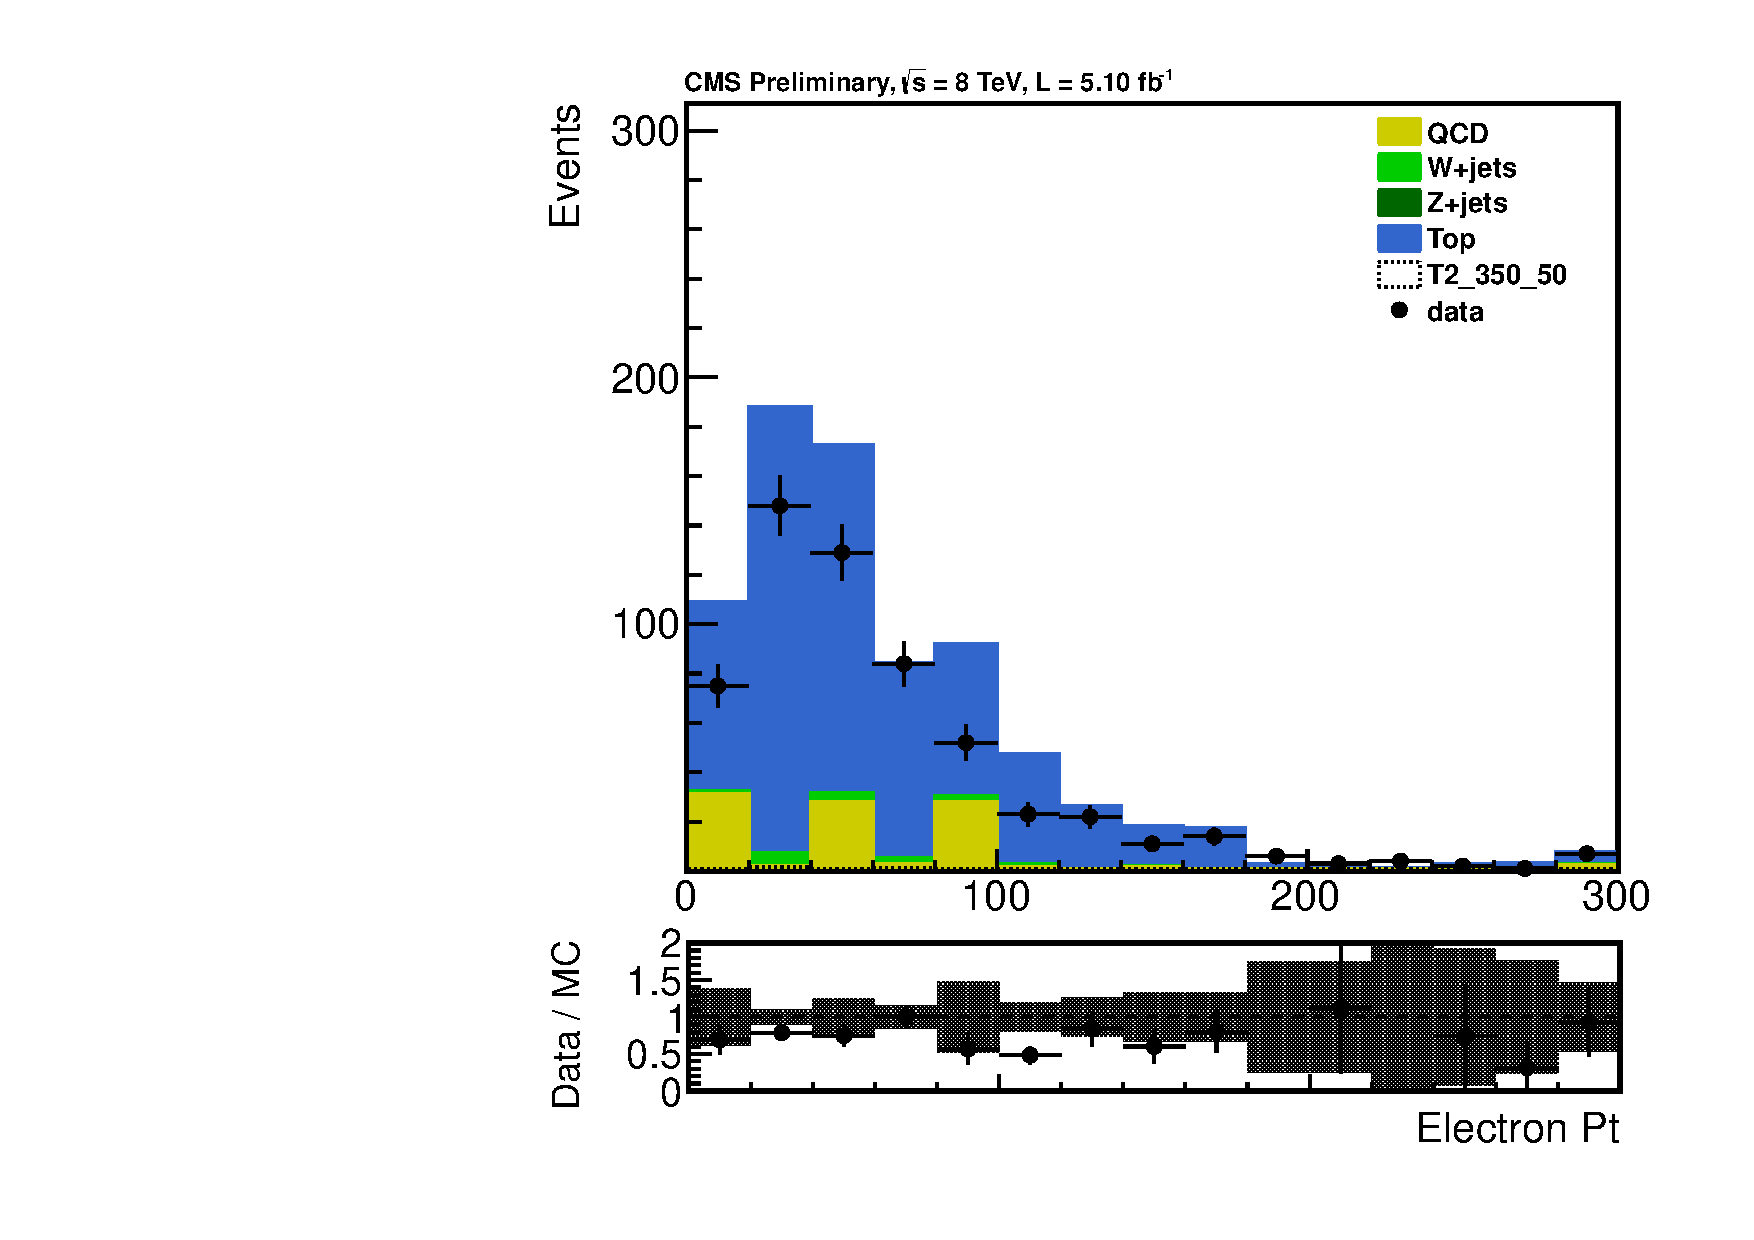
\includegraphics[angle=0,scale=0.39]{myplots/ele_pt.pdf}
%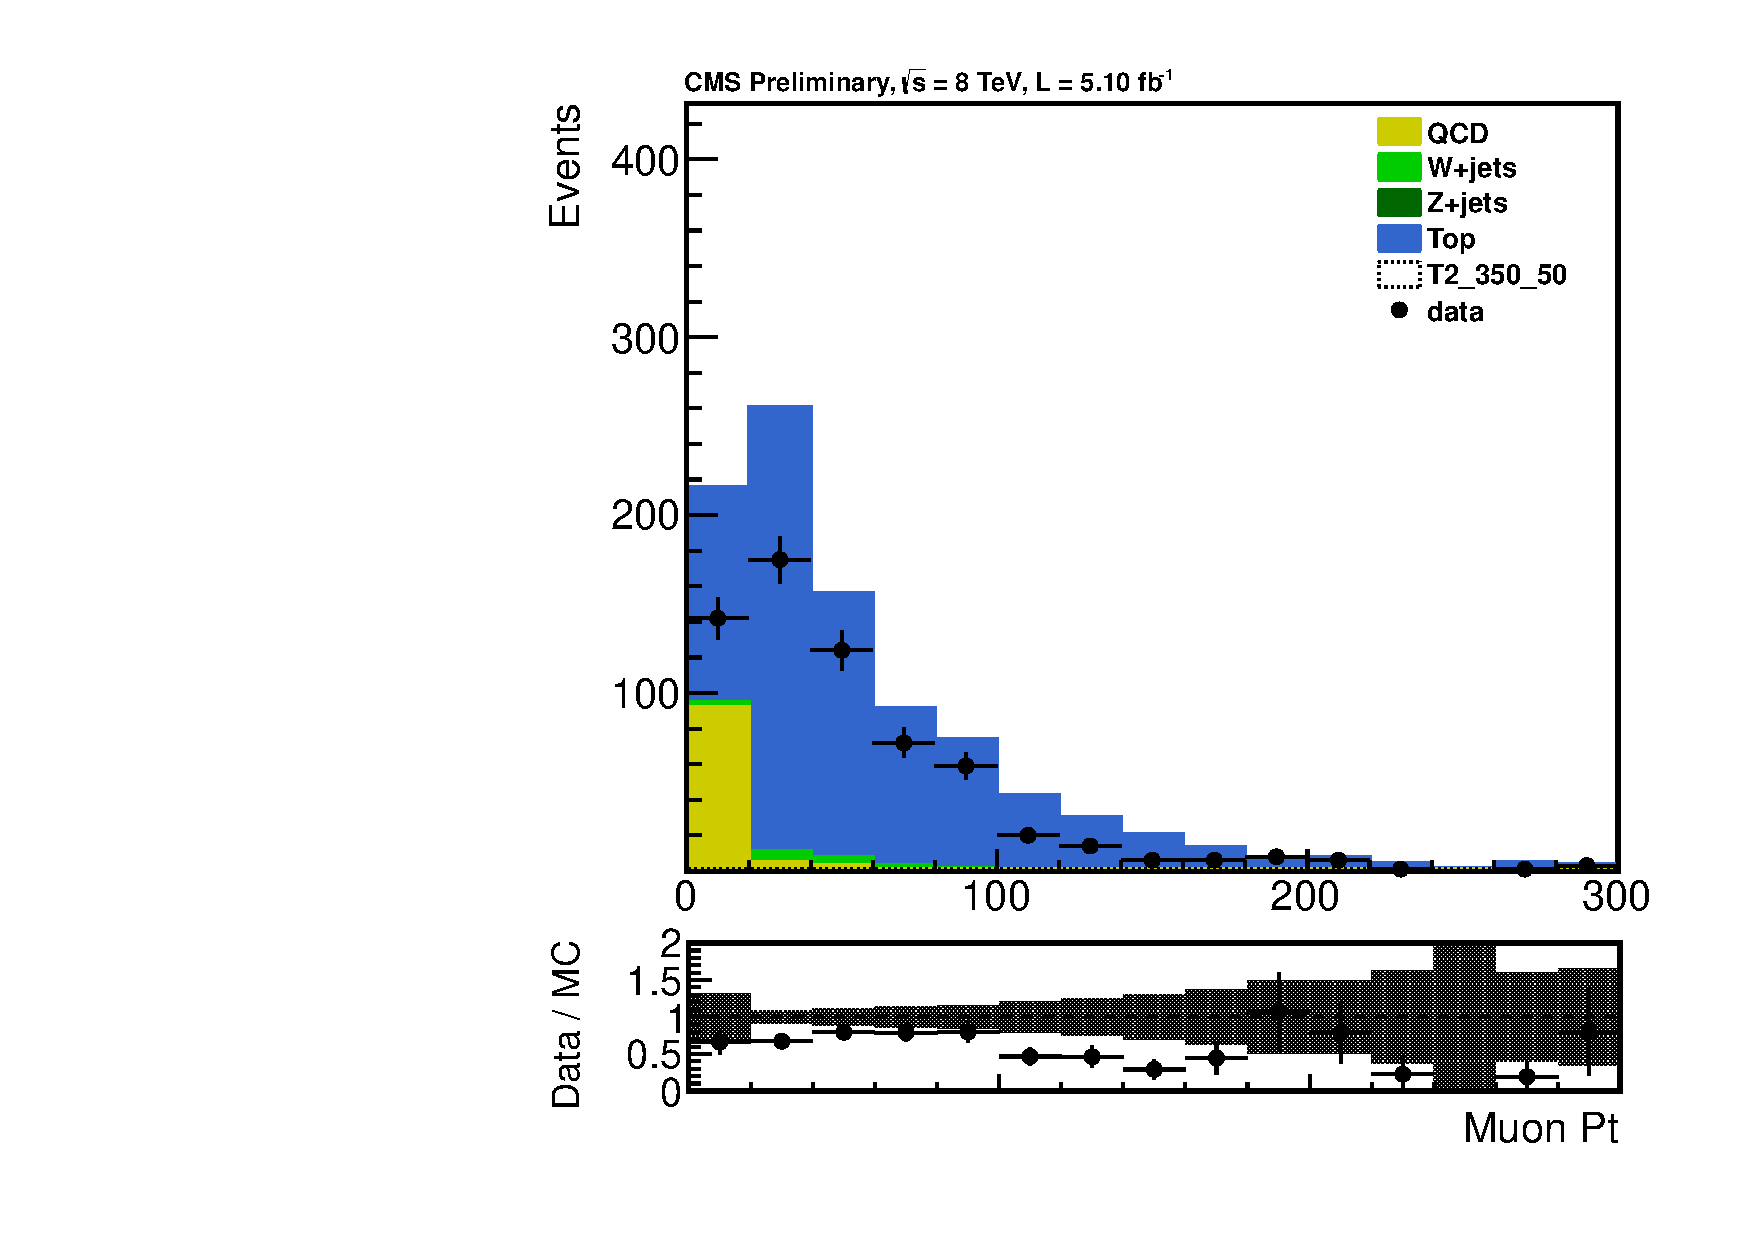
\includegraphics[angle=0,scale=0.39]{myplots/muo_pt.pdf} \\
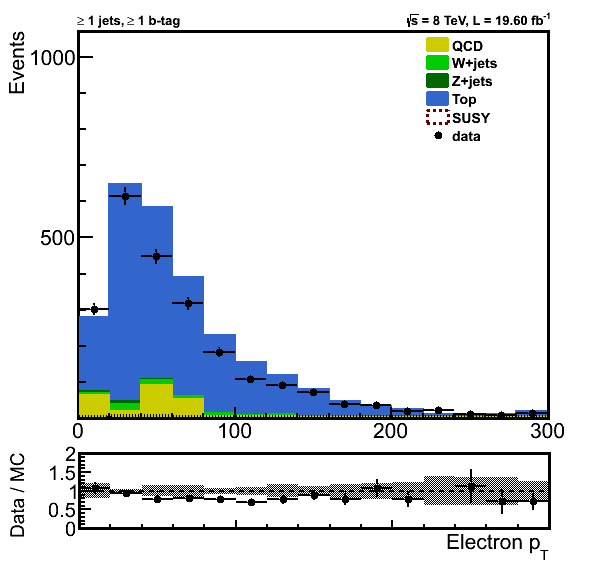
\includegraphics[angle=0,scale=0.35]{llplots_20Invfb/ele_pt.png}
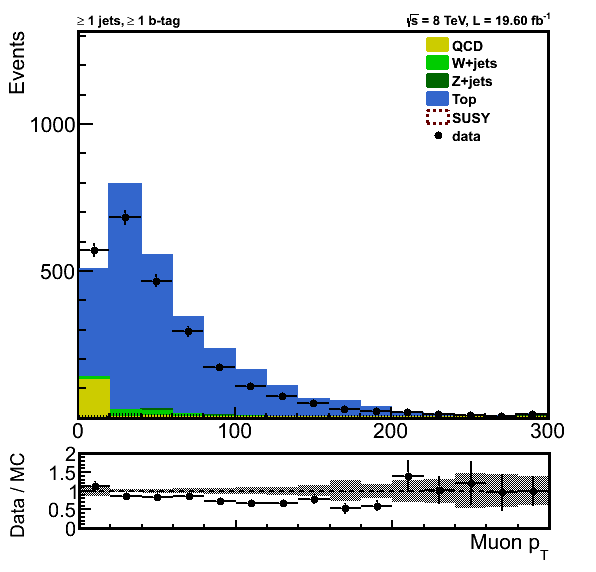
\includegraphics[angle=0,scale=0.35]{llplots_20Invfb/mu_pt.png} \\
\caption{Left: The $p_T$ distribution of the electrons in the events with one electron 
passing all selection cuts but the \mindphifour cut. The reason for this is stated in the text. No $M_{T2}$ cut is applied in 
order to have more statistics. Right: The same plot for muons.}
\label{fig:pt}
\end{figure}

In order to increase the data statistics, the cut on the 
\mindphifour is relaxed. While this cut was introduced in the main analysis to suppress the $QCD$ background events, now that 
the lepton veto is reversed and exactly one lepton is required, the $QCD$ events are still under control. 
Hence relaxing the \mindphifour cut would not be harmful. The only thing which should be taken into account 
is to consider the efficiency of this cut, called as $f$, which is explained in the following.\\
The contribution of the lost lepton background events passing the lepton veto, shown as $N_l^{pass}$, is estimated with the following formula
\begin{eqnarray} 
N_l^{pass}&=&(N_l^{reco}-N_l^{bg})\frac{1}{\varepsilon_l}-(N_l^{reco}-N_l^{bg})\\\nonumber
&=&(N_l^{reco}-N_l^{bg})\frac{1-\varepsilon_l}{\varepsilon_l},\nonumber
\end{eqnarray}
where $N_l^{reco}$ refers to the number of data events with all selection cuts but the inverted 
lepton veto, which requires exactly one lepton. For this set of cuts, the number of background events from processes 
other than $W\rightarrow l\nu_l$ is represented by $N_l^{bg}$ and is taken from MC. The $\varepsilon_l$ contains 
the efficiency for a generated $W\rightarrow l\nu_l$ passing all selection cuts but the inverted lepton veto to have a 
lepton reconstructed. Here, the electron and muon efficiencies are obtained from both $t\bar t$ and $W+jets$ events and a relative contribution is used in the above formula. It should also be noted that, at the generator level, those $t\bar t$ events containing a tau lepton decaying hadronically are vetoed since these kind of events are considered when backgrounds from tau are estimated.\\ 
In order to reduce the signal contamination in the leptonic signal region, a cut on the transverse mass of the 
lepton, $m_T$, is applied which is defined as
$$m_T=\sqrt{2p_T(e,\mu)E_T^{miss}(1-\cos(\Delta\Phi))} < 100\; \rm GeV,$$
where $\Delta\Phi$ is the angle between lepton-$p_T$ and $E_T^{miss}$ in the transverse plane. 
In the $W\rightarrow l\nu_l$ events, the $m_T$ cut represents the transverse mass of 
the $W$ bosons which decreases above $80$ GeV. Hence the leptonic signal events are not 
affected by this cut, while the contamination from SUSY events are strongly suppressed. The 
distribution of the $m_T$ of either electrons or muons in the events with exactly one electron and one muon respectively, are shown in
Figure~\ref{fig:mt}. In this analysis, 
it is found that, e.g. for electron $m_T$ distribution, the $S/B$ decreases from $1.03\%$ to $0.60\%$ when $m_T<100$ GeV cut is introduced. In 
the rest of this section, in addition to all selection cuts, the leptons are required to pass $m_T<100$ GeV cut.\\ 
\begin{figure}[htbp] 
\centering
%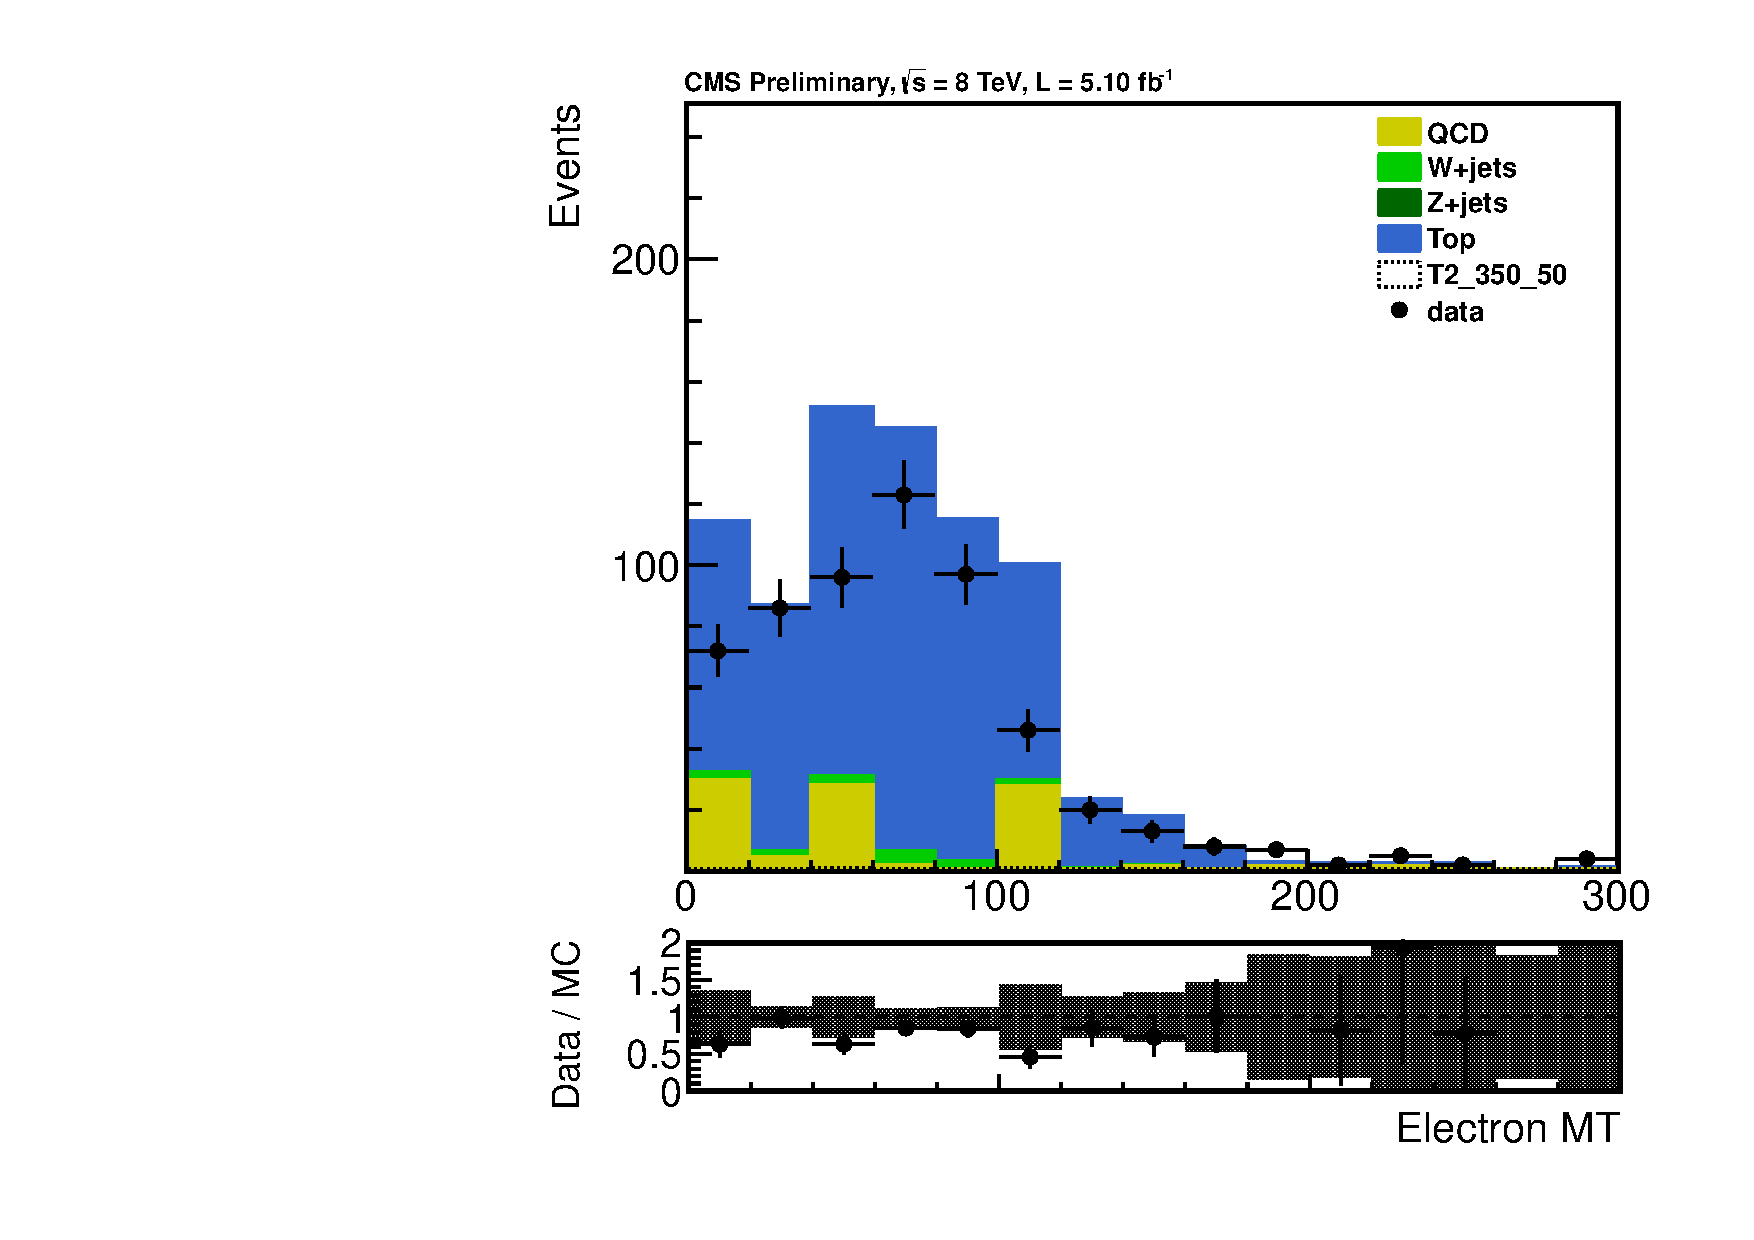
\includegraphics[angle=0,scale=0.39]{myplots/ele_mt.pdf} 
%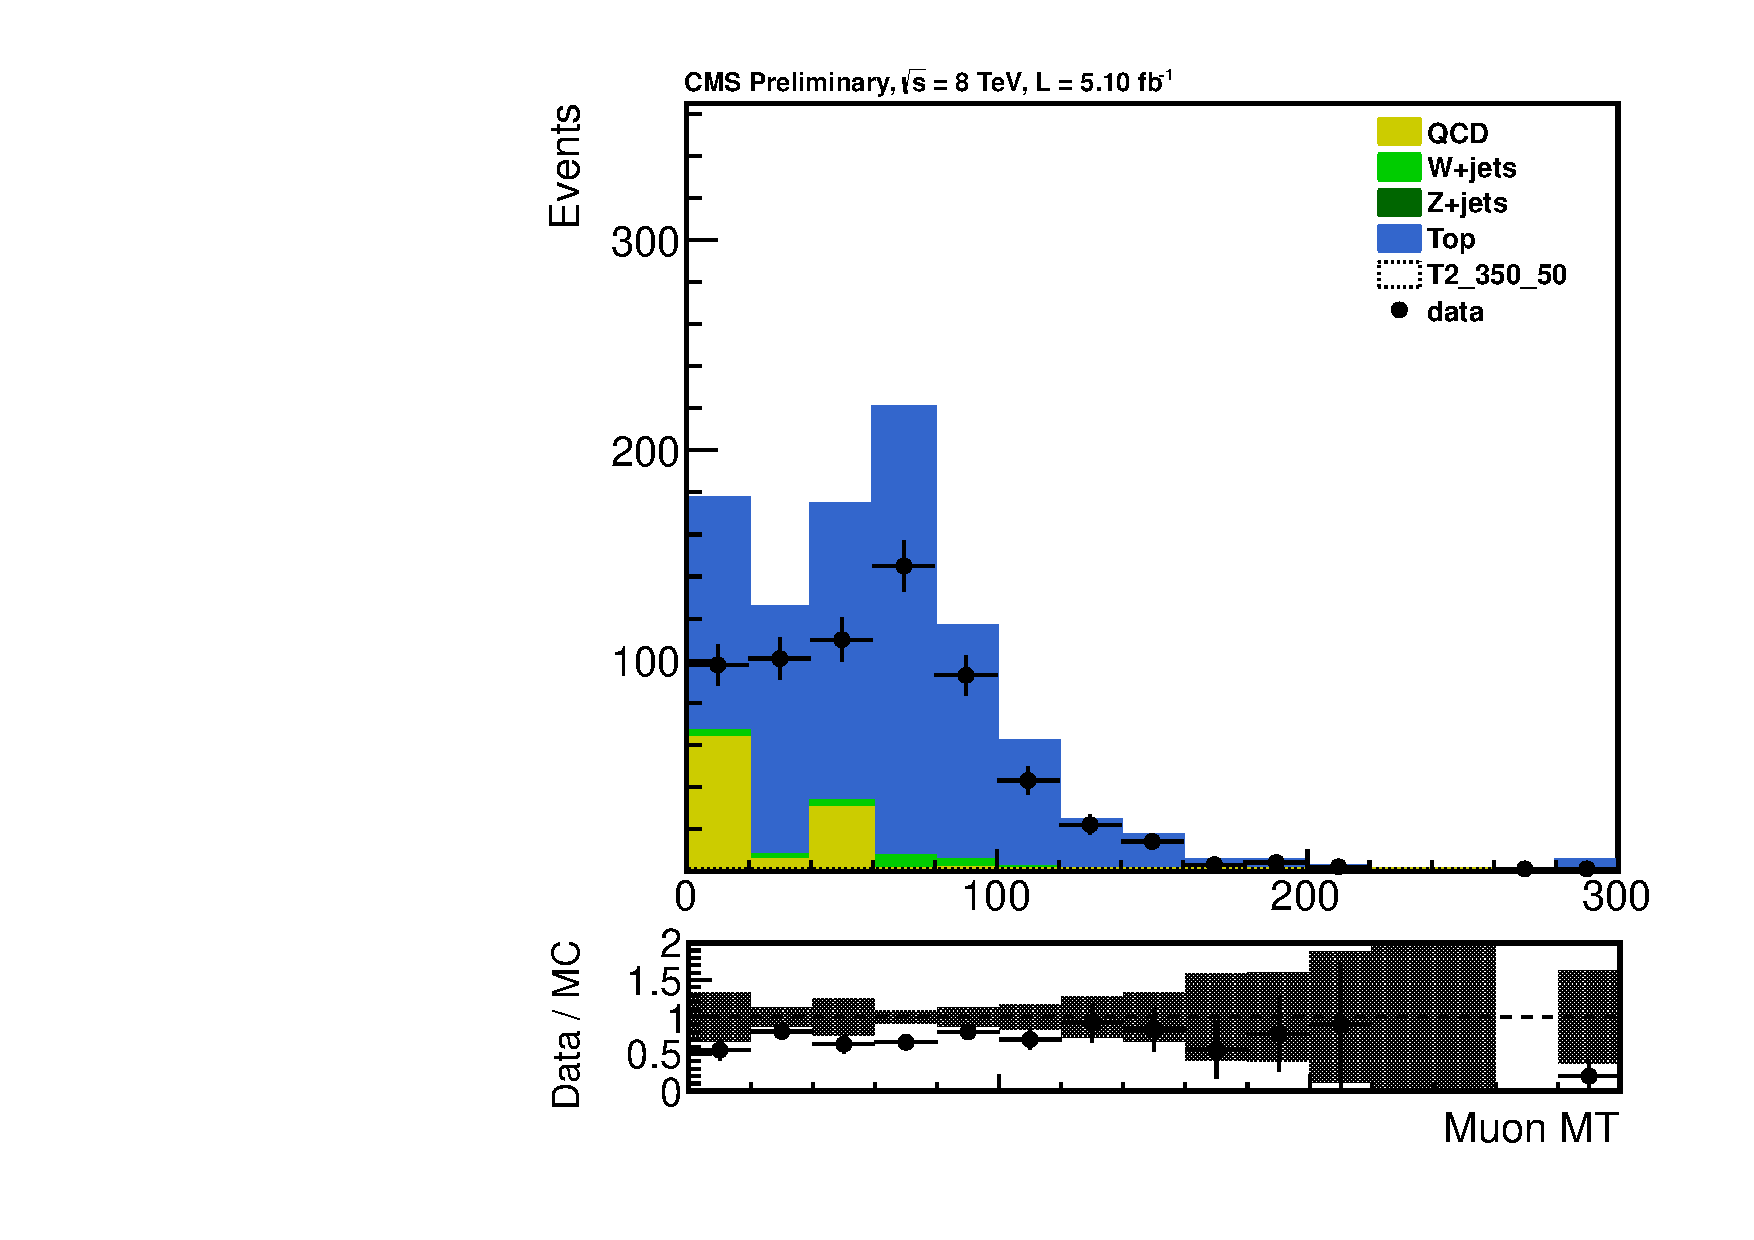
\includegraphics[angle=0,scale=0.39]{myplots/muo_mt.pdf} \\
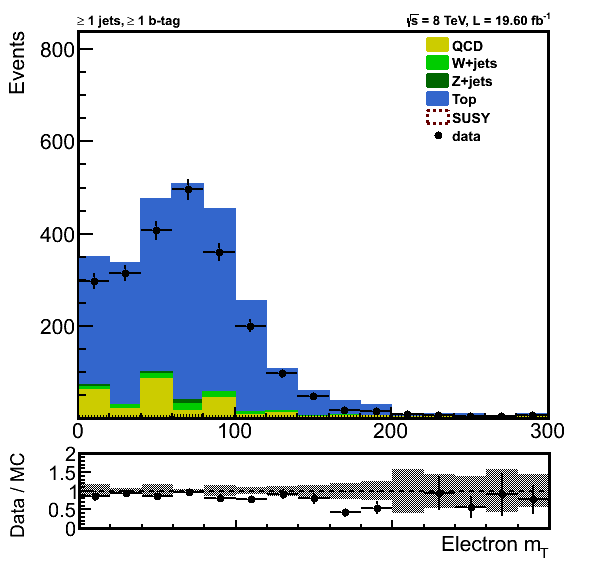
\includegraphics[angle=0,scale=0.35]{llplots_20Invfb/ele_mt.png} 
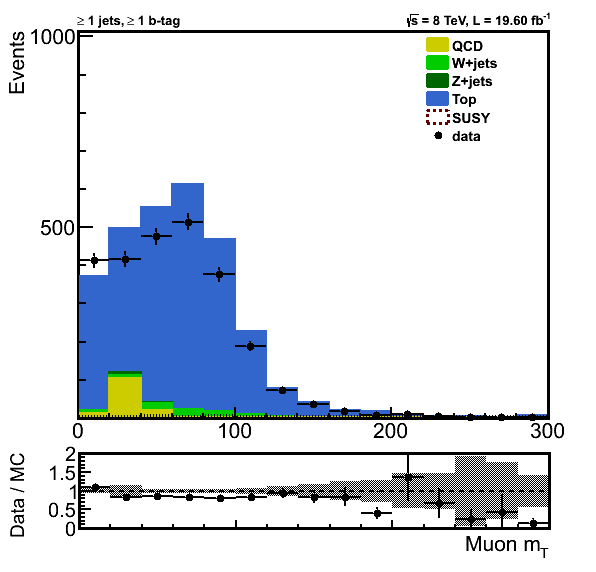
\includegraphics[angle=0,scale=0.35]{llplots_20Invfb/mu_mt.png} \\
\caption{Left: The $m_T$ distribution of the electrons for the events with one electron 
passing all selection cuts but the \mindphifour cut. The reason for this is stated in the text. No $M_{T2}$ cut is applied in 
order to have more statistics. Right: The same plot for muons.}
\label{fig:mt}
\end{figure}

The fraction of events with all selection cuts with respect to the events with all 
selection cuts but the \mindphifour are shown 
in Figure~\ref{fig:fraction} for data and MC. Since in the signal region, defined as region with $M_{T2}>125$ GeV, the ratios become flat; therefore one can fit the ratios with a straight line. For both electrons and muons, the MC ratio is fitted and the fitted parameters $f$ are quoted in Table~\ref{tbl:fitvalues}.\\
\begin{figure}[htbp] 
\centering
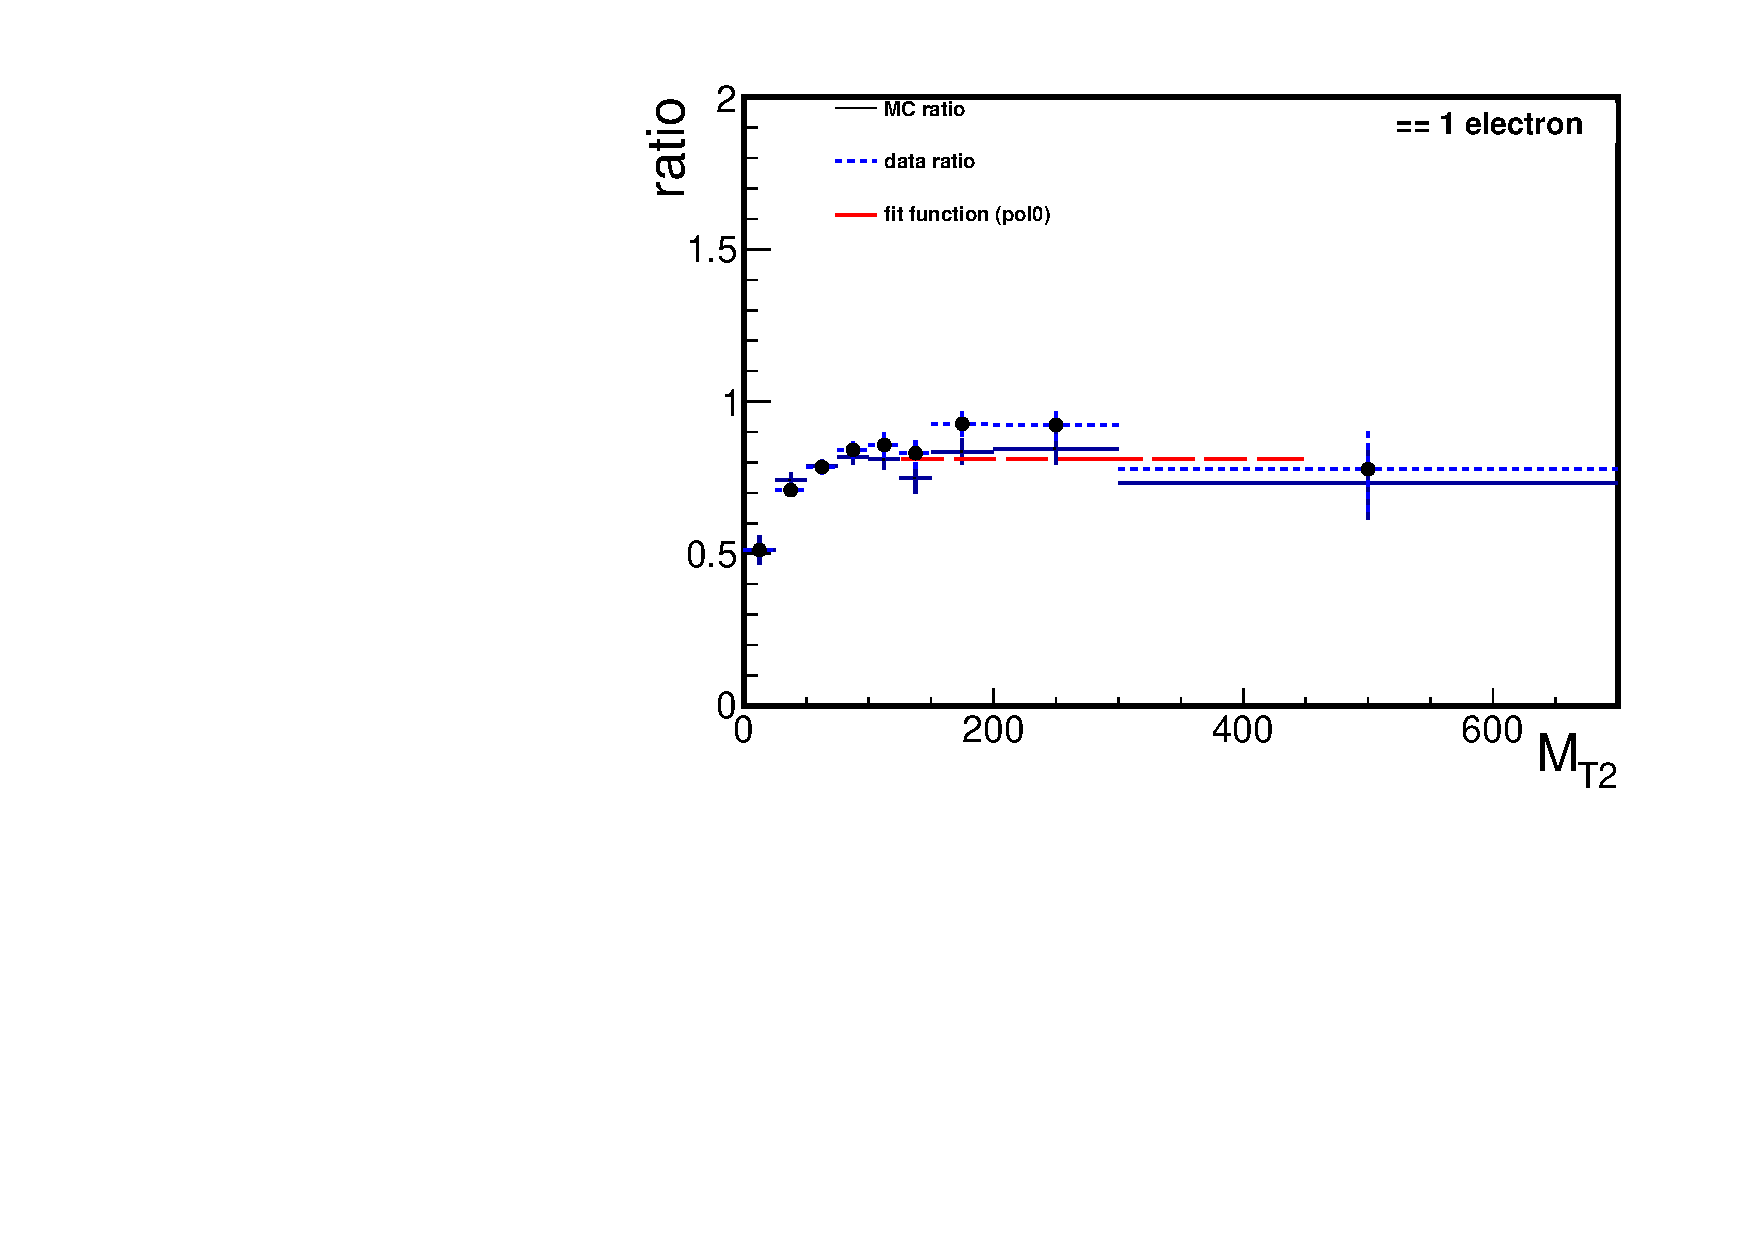
\includegraphics[angle=0,scale=0.39]{llplots_20Invfb/ele_ratio.pdf} 
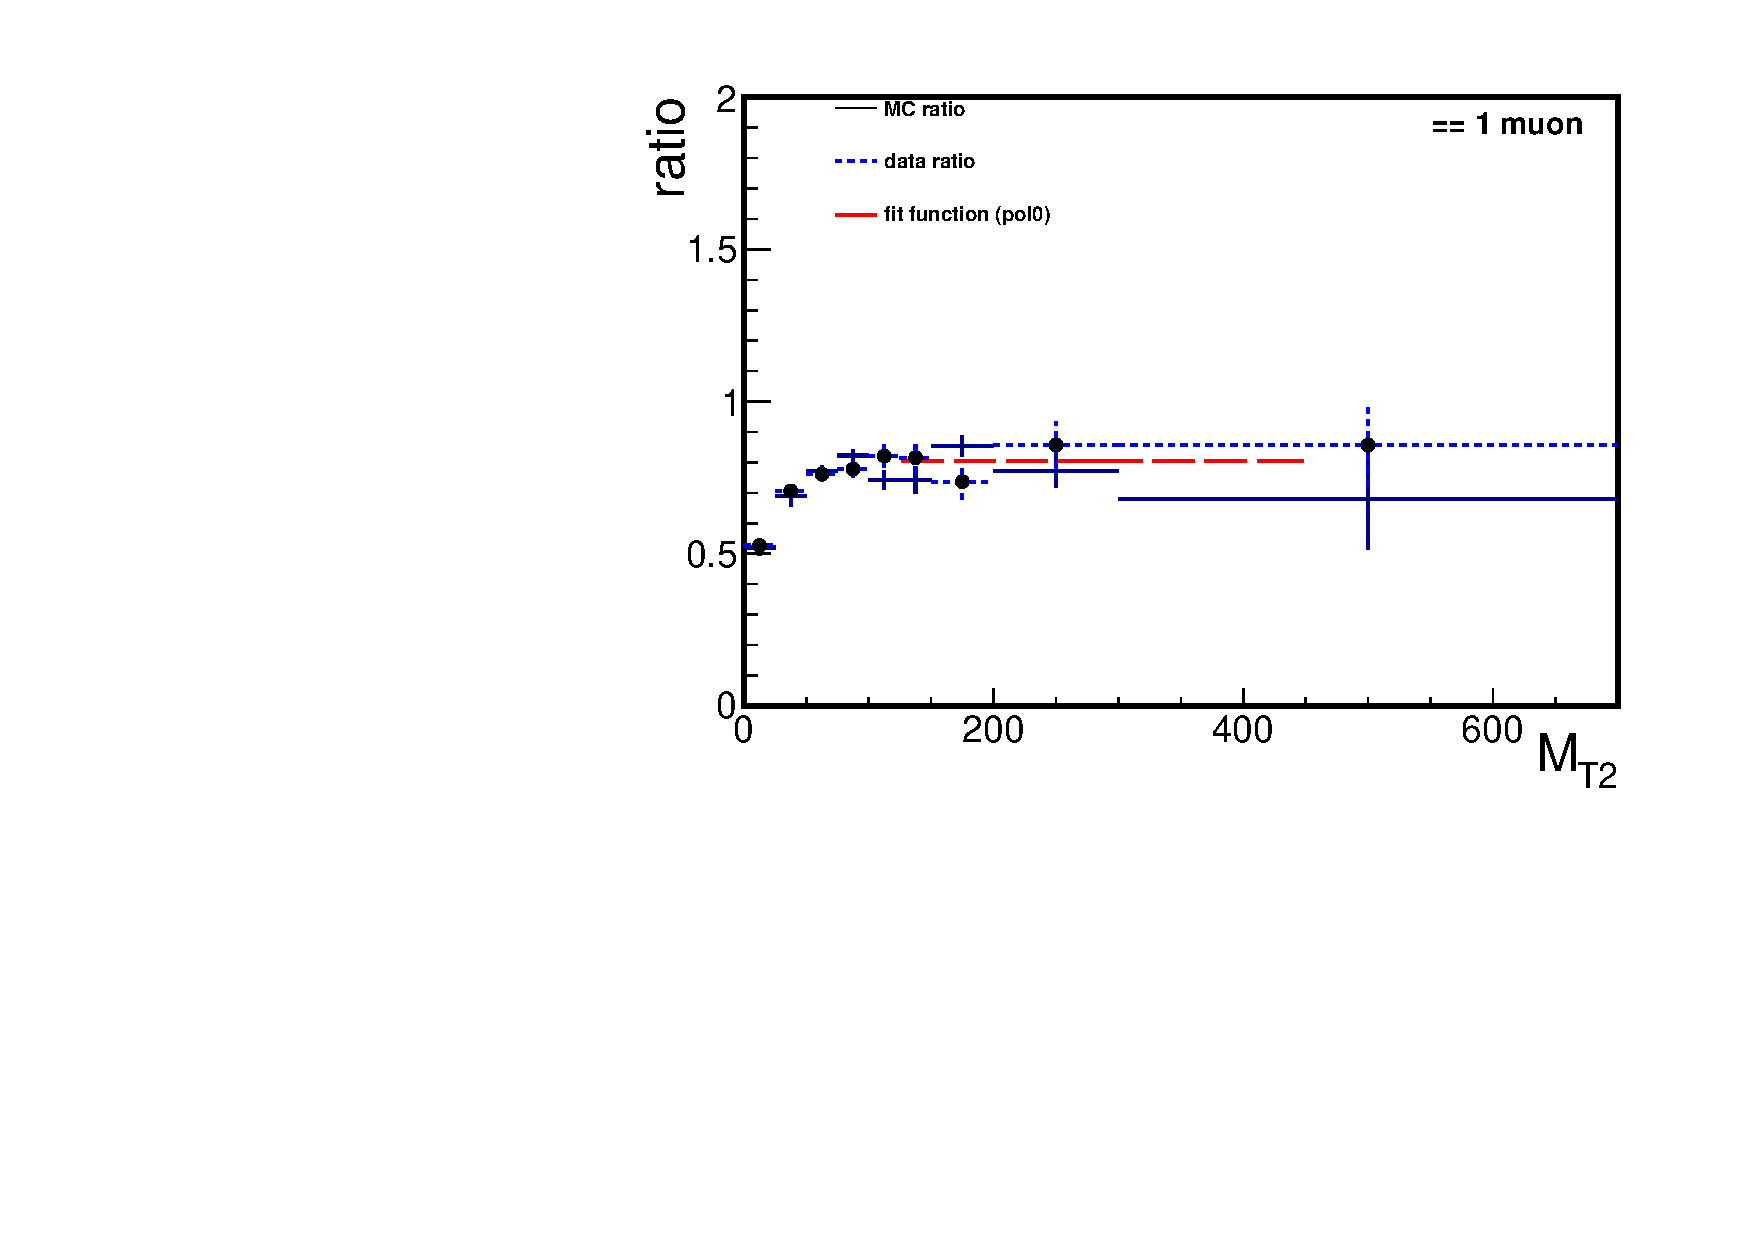
\includegraphics[angle=0,scale=0.39]{llplots_20Invfb/mu_ratio.pdf} \\
\caption{Left: Ratio between events with one electron passing all selection cuts 
versus events with one electron passing all selection cuts but the 
\mindphifour for data (blue) and MC (black). 
The fit line for the MC ratio over all $M_{T2}$ signal bins is drawn in red. Right: The same plot for events with one muon.}
\label{fig:fraction}
\end{figure}

\begin{table}[hbtp]
\begin{center}
\small
\begin{tabular}{lcc}\hline\hline
   &  electrons    &   muons   \\ \hline
Fit value for the ratio $f$    & $0.811 \pm 0.028$     &   $0.804 \pm 0.024$    \\ \hline\hline
\end{tabular}
\caption{Fit values $f$ obtained from the MC ratios for electrons and muons.}
\label{tbl:fitvalues}
\end{center}
\end{table}

The results of estimation of the lost lepton background events from data are summarized in 
Table~\ref{tbl:llestimation}. It should be mentioned that, the number of data events with 
one lepton selection and its corresponding background events are obtained from the relaxed 
cut selection, where \mindphifour is dropped. Therefore the prediction 
is corrected back by multiplying the event yield with the fitted ratio value $f$.\\ 
\begin{table}[hbtp]
\begin{center} 
\begin{tabular}{lccccc} 
\hline\hline 
& %$N^{W,Top}$ MC &
 $N^{reco}$ & $N^{bg}$ & $R_{LL}$ & $N^{pass}$ MC-Truth & $N^{pass}$ data-prediction \\\hline 
electrons &%&
&&&&\\\hline 
& %$38.94$ &
 $129$ & $20.78$ & $1.18\pm0.20$ & $148.99\pm 9.66$ & $127.82\pm 13.41(stat)\pm 32.41(sys)$\\\hline\hline 
muons &%&
&&&&\\\hline 
& %$45.55$ &
 $150$ & $26.04$ & $0.66\pm0.14$ & $105.23\pm 8.14$ & $81.90\pm 8.09(stat)\pm 24.29(sys)$\\  
\hline\hline 
\end{tabular} 
\caption{Data-Driven Estimation of Lost Lepton from $W+$jets and $t(\bar t)$ for electrons and muons. The lost lepton ratio $R_{LL}$ is given by $f\frac{1-\varepsilon_l}{\varepsilon_l}$.}
\label{tbl:llestimation}
\end{center} 
\end{table} 

It should be noted that for the systematic uncertainty, two possible sources are taken into account. A first one is a systematic uncertainty of 100\% on the number of backgrounds. A second one is a systematic uncertainty of 5\%, considered when calculating the efficiencies $\varepsilon_l$ from MC, to account for possible difference between data and simulation.
